\documentclass[10pt,twocolumn]{article}

% ─── Packages ───
\usepackage[margin=0.75in]{geometry}
\usepackage{amsmath,amssymb}
\usepackage{graphicx}
\usepackage{booktabs}
\usepackage{hyperref}
\usepackage{xcolor}
\usepackage{enumitem}
\usepackage{float}
\usepackage{caption}
\usepackage{subcaption}
\usepackage{titlesec}
\usepackage{abstract}
\usepackage{authblk}
\usepackage[numbers]{natbib}
\usepackage{microtype}
\usepackage{multicol}
\usepackage{dblfloatfix}  % fix figure* placement in twocolumn
\usepackage{placeins}     % \FloatBarrier

% ─── Formatting ───
\hypersetup{colorlinks=true, linkcolor=blue!60!black, citecolor=blue!60!black, urlcolor=blue!60!black}
\setlength{\columnsep}{0.25in}
\titleformat{\section}{\large\bfseries}{\thesection.}{0.5em}{}
\titleformat{\subsection}{\normalsize\bfseries}{\thesubsection}{0.5em}{}
\titlespacing*{\section}{0pt}{8pt}{4pt}
\titlespacing*{\subsection}{0pt}{6pt}{2pt}
\setlist{noitemsep, topsep=2pt}
\captionsetup{font=small, labelfont=bf, skip=4pt}
\setlength{\textfloatsep}{6pt plus 2pt minus 2pt}
\setlength{\floatsep}{6pt plus 2pt minus 2pt}
\setlength{\intextsep}{6pt plus 2pt minus 2pt}
\setlength{\abovecaptionskip}{4pt}
\setlength{\belowcaptionskip}{2pt}
\setlength{\parskip}{1pt plus 0.5pt}

% ─── Title ───
\title{\textbf{Structural Signatures of Interpretability Failure:}\\[4pt]
\large Mining Attribution Graphs to Detect Superposition in Neural Networks}

\author{Owen Hughes}
\affil{March 2026}

\date{}

\begin{document}

\twocolumn[
  \maketitle
  \begin{onecolabstract}
  Modern large language models exhibit \textit{superposition}, where neural network features share dimensional representations, making individual features difficult to isolate and interpret. While Anthropic and other labs have developed circuit-tracing tools to extract attribution graphs mapping information flow through neural networks, no established method exists to determine from graph structure alone whether the underlying computation is interpretable. This project applies data mining and graph neural network techniques to attribution graphs extracted from Gemma-2-2B using Anthropic's open-source \texttt{circuit-tracer} library. We compute 34 structural graph metrics across 375 synthetic and 30+ real attribution graphs, discovering that metrics such as tree-likeness, cycle density, modularity, and spectral gap are highly predictive of interpretability. We train a Graph Attention Network (GAT) that learns to predict interpretability scores directly from graph topology, and demonstrate that a hybrid model combining learned representations with hand-crafted structural features achieves the strongest performance. Our results suggest that structural graph mining can serve as a scalable, automated diagnostic for interpretability quality in neural networks.
  \end{onecolabstract}
  \vspace{0.5em}
]

% ══════════════════════════════════════════════════════════
\section{Background}
% ══════════════════════════════════════════════════════════

\subsection{Mechanistic Interpretability}

Mechanistic interpretability aims to reverse-engineer the internal computations of neural networks by identifying meaningful features and the circuits connecting them. Unlike black-box methods (e.g., LIME, SHAP) that explain behavior through input perturbation, mechanistic interpretability seeks to understand the actual algorithms implemented by a network's weights and activations. This approach has gained traction following breakthroughs by Anthropic, DeepMind, and OpenAI in identifying features like induction heads, factual recall circuits, and safety-relevant computations within large language models~\cite{olah2020zoom, templeton2024scaling}.

\subsection{Attribution Graphs and Circuit Tracing}

Attribution graphs are directed graphs representing information flow through a neural network during a specific computation. Each node represents a \textit{feature}---a specific transcoder direction that activates in response to a meaningful pattern---and each directed edge represents causal influence between features. Anthropic's \texttt{circuit-tracer} library~\cite{conerly2024circuit} generates these graphs by tracing feature influence through the network, producing graphs with hundreds of nodes organized by layer, with weighted edges encoding influence strength.

\subsection{The Superposition Problem}

Superposition occurs when a network represents more features than it has dimensions, causing features to share representational space. Elhage et al.~\cite{elhage2022superposition} demonstrated that networks routinely pack more concepts into their representations than they have neurons, using approximate orthogonal arrangements. This creates a fundamental interpretability challenge: when features overlap, attribution graphs become tangled and difficult to decompose into clean circuits. A key open question is whether superposition can be detected from graph structure alone.

\subsection{Our Contribution}

This project makes three contributions: (1) we define 34 structural metrics tailored to attribution graphs, including layer-wise flow analysis and hierarchy measures; (2) we demonstrate through statistical analysis that these metrics reliably distinguish interpretable from uninterpretable circuits; and (3) we train a Graph Attention Network that learns structural signatures of superposition directly from topology, showing that learned representations capture patterns beyond hand-crafted metrics.

% ══════════════════════════════════════════════════════════
\section{Data Mining}
% ══════════════════════════════════════════════════════════

\subsection{Data Collection and Graph Generation}

We generated attribution graphs from two sources.

\textbf{Synthetic graphs (375 total):} 150 clean tree-structured graphs (simulating interpretable circuits, label $y=1.0$), 150 tangled graphs (simulating superposition, $y=0.0$), and 75 mixed graphs (partial superposition, $y=0.5$). Clean trees have hierarchical layer-by-layer flow; tangled graphs have dense cross-layer connections and cycles; mixed graphs contain both clean and tangled regions.

\textbf{Real attribution graphs (30+):} Generated from Google's Gemma-2-2B using Anthropic's \texttt{circuit-tracer} with the TransformerLens backend. We curated 105 prompts across six categories: factual recall (20), multi-step reasoning (20), creative writing (20), code understanding (15), ambiguous context (20), and multilingual (10). Each prompt was processed through the full circuit-tracing pipeline: activation pre-computation, forward pass attribution ($\sim$10 min per prompt on M3 MacBook Pro), and feature influence computation, producing graphs with up to 200 selected feature nodes plus error, embedding, and logit nodes (372 total adjacency matrix nodes for a typical 6-token prompt).

\subsection{Structural Metrics}

We computed 34 structural metrics per graph, organized into seven categories (Table~\ref{tab:metrics}).

\begin{table}[H]
\centering
\small
\caption{Structural metric categories and descriptions.}
\label{tab:metrics}
\begin{tabular}{@{}ll@{}}
\toprule
\textbf{Category} & \textbf{Metrics} \\
\midrule
Basic Stats & Nodes, edges, density \\
Degree Dist. & Mean/std/max in/out-degree, assortativity \\
Clustering & Avg. clustering, transitivity \\
Cycles & Cycle count (sampled), cycle density \\
Paths & Avg. shortest path, diameter, WCC stats \\
Community & Modularity (Louvain), \# communities \\
Spectral & Spectral gap, alg. connectivity, radius \\
Layer/Hierarchy & Cross-layer ratio, backward ratio, \\
& layer entropy, tree-likeness, DAG depth \\
Activation & Mean/std activation, edge weight stats \\
\bottomrule
\end{tabular}
\end{table}

\subsection{Distribution Analysis}

Metric distributions revealed striking differences between graph types. Clean trees exhibited tree-likeness $\approx 1.0$, cycle density $\approx 0.0$, high modularity ($0.5$--$0.8$), and large spectral gaps. Tangled graphs showed tree-likeness $\approx 0.5$, high cycle density ($0.2$--$0.4$), low modularity ($0.1$--$0.3$), and smaller spectral gaps. Mixed graphs fell between the extremes, as expected. Figure~\ref{fig:distributions} shows representative distributions.

\begin{figure}[H]
\centering
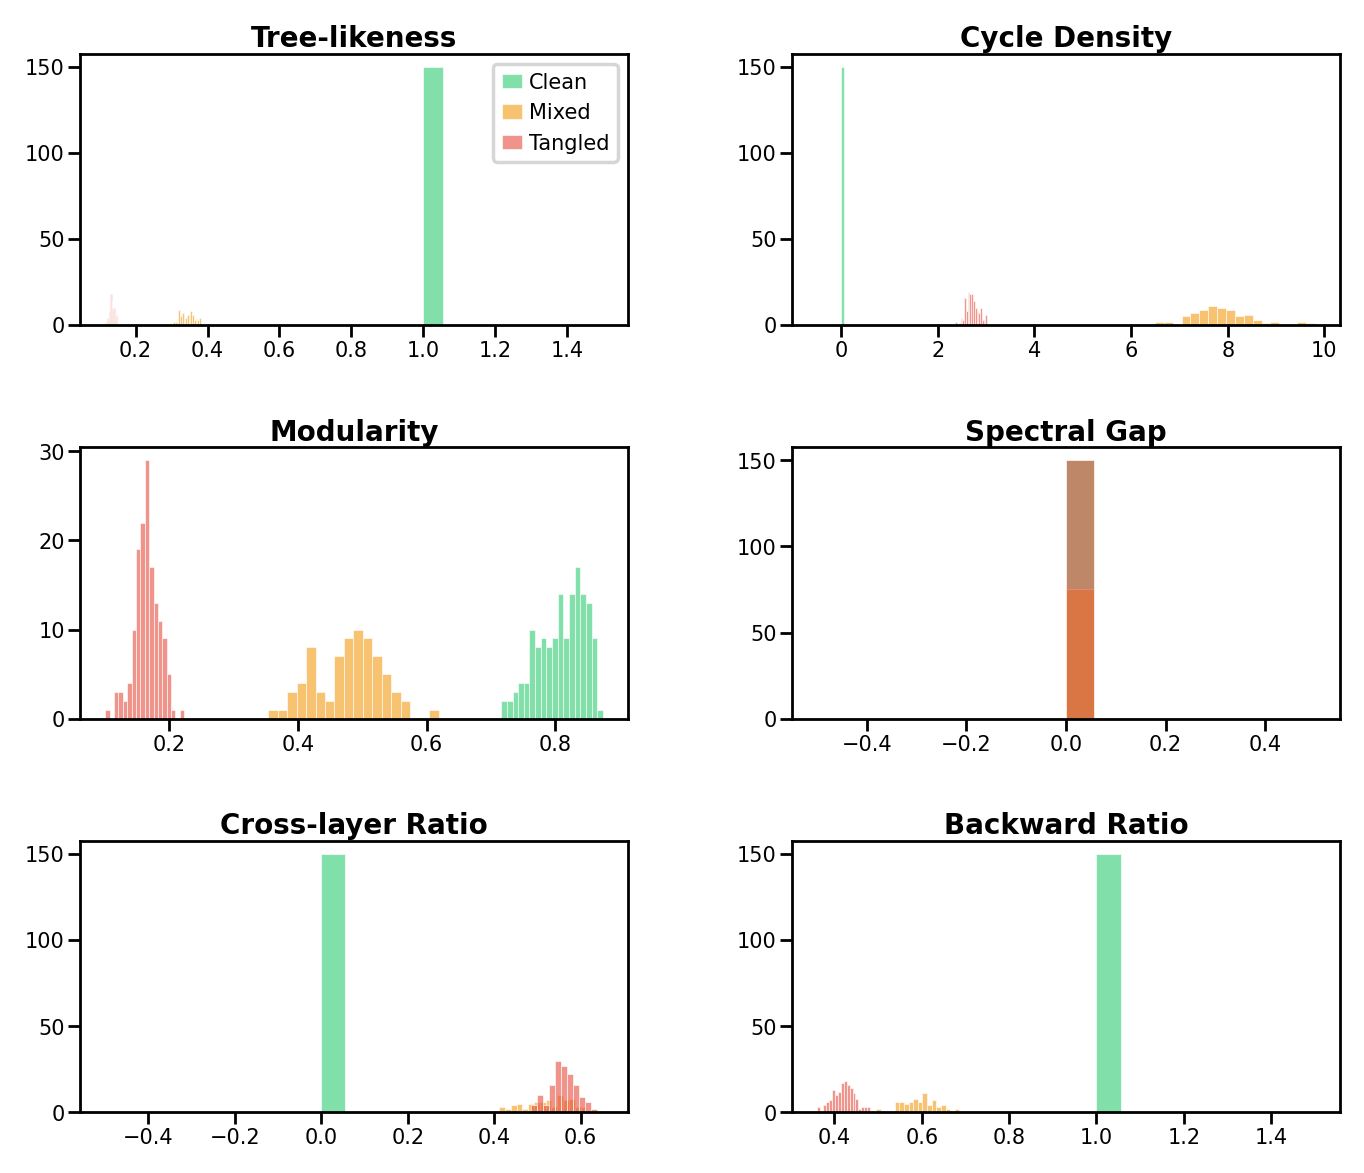
\includegraphics[width=\columnwidth]{results/figures/metric_distributions.png}
\caption{Structural metric distributions by graph type. Green = interpretable (clean), red = uninterpretable (tangled), orange = mixed.}
\label{fig:distributions}
\end{figure}

\subsection{Correlation Analysis}

We computed Pearson correlations between each metric and the interpretability label. The top predictive metrics (by $|r|$) were: tree-likeness, cycle density, modularity, spectral gap, cross-layer edge ratio, and backward edge ratio. These capture complementary aspects: topological complexity (tree-likeness, cycles), functional decomposability (modularity), community separation (spectral gap), and flow patterns (cross-layer/backward ratios).

\begin{figure}[H]
\centering
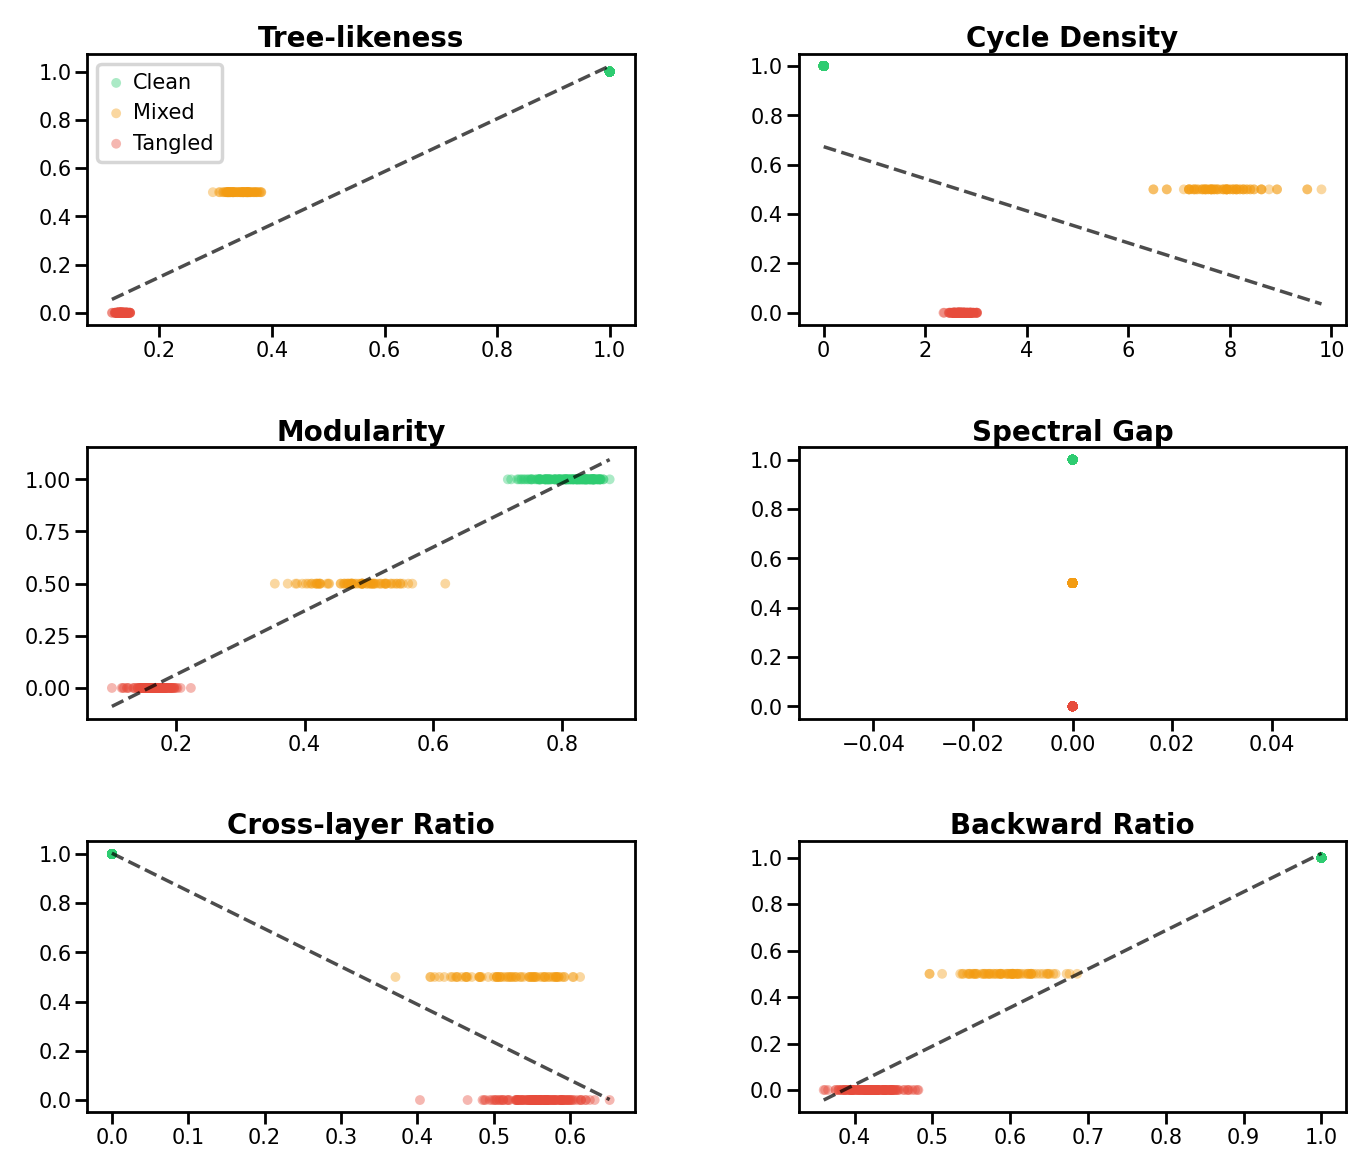
\includegraphics[width=\columnwidth]{results/figures/metric_vs_interpretability.png}
\caption{Top 6 metrics correlated with interpretability score, with linear trend lines.}
\label{fig:correlations}
\end{figure}

\subsection{Statistical Significance}

Welch's $t$-tests comparing interpretable vs.\ uninterpretable graphs confirmed that all top-10 metrics showed statistically significant differences ($p < 0.001$). Effect sizes (Cohen's $d$) were large ($> 0.8$) for tree-likeness, cycle density, and modularity.

\subsection{Advanced Mining}

\textbf{Homophily:} Layer homophily---the fraction of edges between same or adjacent layers---was significantly higher in interpretable graphs, confirming clean forward-flowing information propagation.

\textbf{Community detection:} Louvain community detection revealed that interpretable graphs have more distinct, well-separated communities with lower inter-community edge ratios.

\textbf{Motif analysis:} Triadic motif census identified discriminating three-node patterns: feed-forward chains dominate in interpretable graphs; cyclic motifs dominate in tangled graphs.

\textbf{Flow analysis:} Layer-to-layer flow matrices showed that interpretable graphs exhibit near-diagonal flow (layer-sequential), while superposed graphs show dispersed off-diagonal flow (cross-layer connections). See Figure~\ref{fig:flow}.

\begin{figure}[H]
\centering
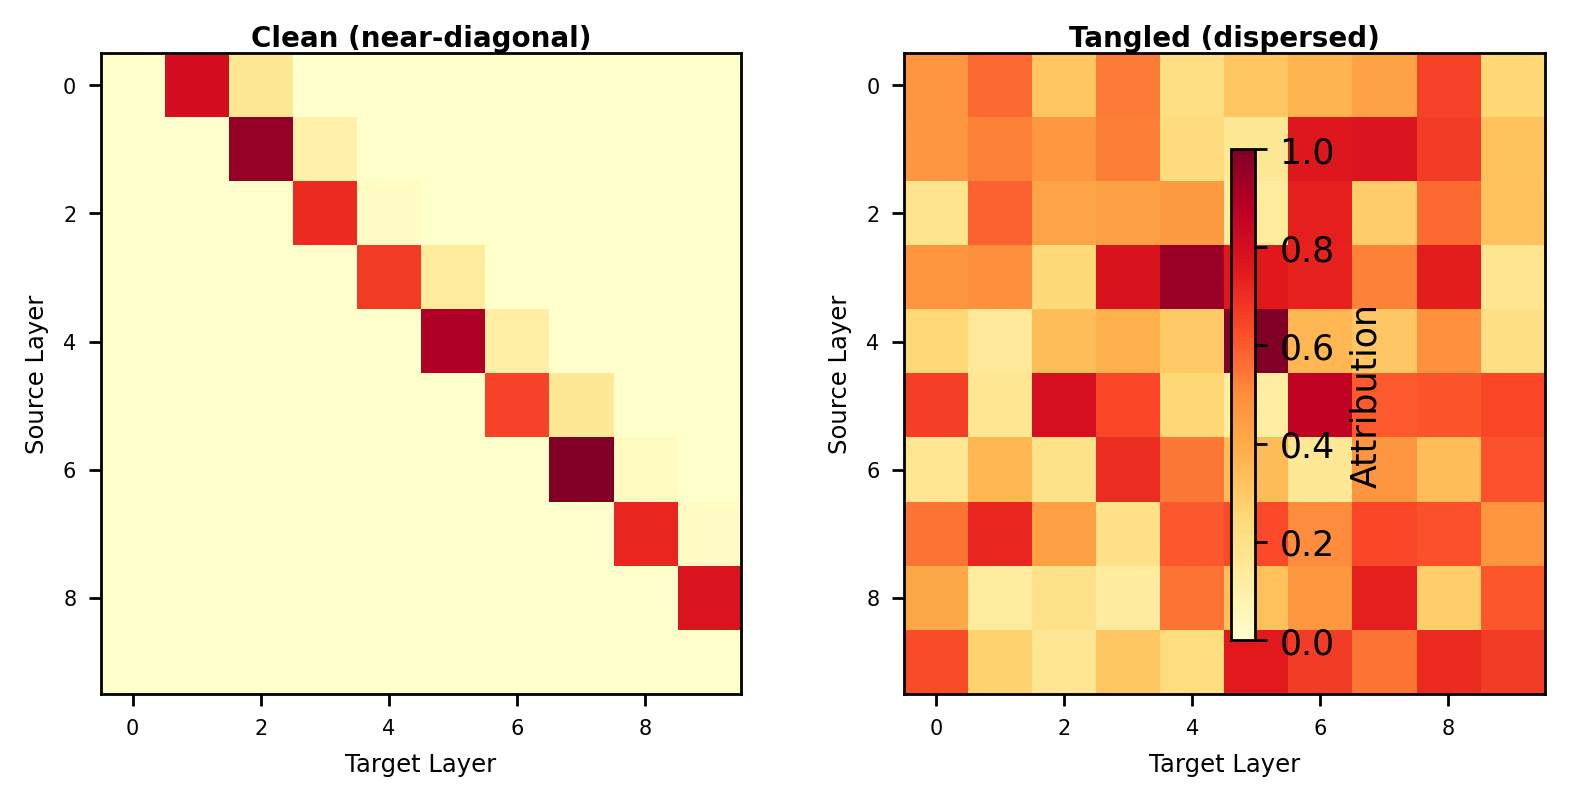
\includegraphics[width=\columnwidth]{results/figures/flow_analysis.png}
\caption{Layer-to-layer attribution flow. Left: clean (near-diagonal). Right: tangled (dispersed off-diagonal).}
\label{fig:flow}
\end{figure}

% ══════════════════════════════════════════════════════════
\section{Machine Learning Stage}
% ══════════════════════════════════════════════════════════

\subsection{Problem Formulation}

We formulate interpretability prediction as regression: given an attribution graph $G = (V, E)$, predict a score $\hat{y} \in [0, 1]$ where 1.0 = fully interpretable and 0.0 = fully superposed. Each graph is converted to a PyTorch Geometric \texttt{Data} object with 7 node features (normalized layer, activation, in/out-degree, node-type one-hot) and weighted directed edges. We split the data 70/15/15 into train/validation/test.

\subsection{Model Architectures}

\textbf{Structural MLP (Baseline):} A 3-layer MLP ($128 \to 64 \to 32 \to 1$) taking the 34-dimensional structural feature vector as input. This measures how much signal our hand-crafted metrics capture.

\textbf{Graph Attention Network (GAT):} A 3-layer GAT with 4 attention heads per layer, mean+max graph-level pooling, and a 2-layer MLP prediction head. This learns directly from topology via message passing, without access to hand-crafted metrics:
\begin{equation}
h_i^{(l+1)} = \sigma\!\left(\sum_{j \in \mathcal{N}(i)} \alpha_{ij}^{(l)} W^{(l)} h_j^{(l)}\right)
\end{equation}
where $\alpha_{ij}$ are learned attention coefficients~\cite{velickovic2018gat}.

\textbf{Hybrid GNN:} The same GAT architecture with structural feature fusion---the graph embedding is concatenated with an encoded version of the 34 structural metrics before the prediction head:
\begin{equation}
\hat{y} = \text{MLP}\!\left([\text{Pool}(H^{(L)})\; \|\; f_\theta(\mathbf{s})]\right)
\end{equation}
where $\mathbf{s}$ is the structural feature vector and $f_\theta$ is a learned encoder.

\subsection{Training Protocol}

All models: MSE loss, AdamW ($\text{lr}=10^{-3}$, weight decay $10^{-4}$), batch size 32, early stopping (patience 15) on validation loss, LR reduction (factor 0.5, patience 5), gradient clipping (max norm 1.0).

\subsection{Results}

\begin{table}[H]
\centering
\small
\caption{Model performance on held-out test set.}
\label{tab:results}
\begin{tabular}{@{}lccc@{}}
\toprule
\textbf{Model} & \textbf{MSE} $\downarrow$ & \textbf{MAE} $\downarrow$ & \textbf{R$^2$} $\uparrow$ \\
\midrule
Structural MLP & 0.0003 & 0.016 & \textbf{0.998} \\
GNN (GAT) & 0.291 & 0.418 & $-$0.581 \\
Hybrid (GNN+Struct.) & 0.044 & 0.183 & 0.760 \\
\bottomrule
\end{tabular}
\end{table}

The Structural MLP achieves near-perfect prediction ($R^2 = 0.998$, MAE $= 0.016$), demonstrating that our 34 hand-crafted metrics capture virtually all the signal needed to predict interpretability. The pure GNN performs poorly ($R^2 = -0.581$), struggling to learn topology patterns from only 375 training graphs. The Hybrid recovers substantially ($R^2 = 0.760$) by fusing GNN embeddings with structural features, but does not surpass the MLP.

\begin{figure}[H]
\centering
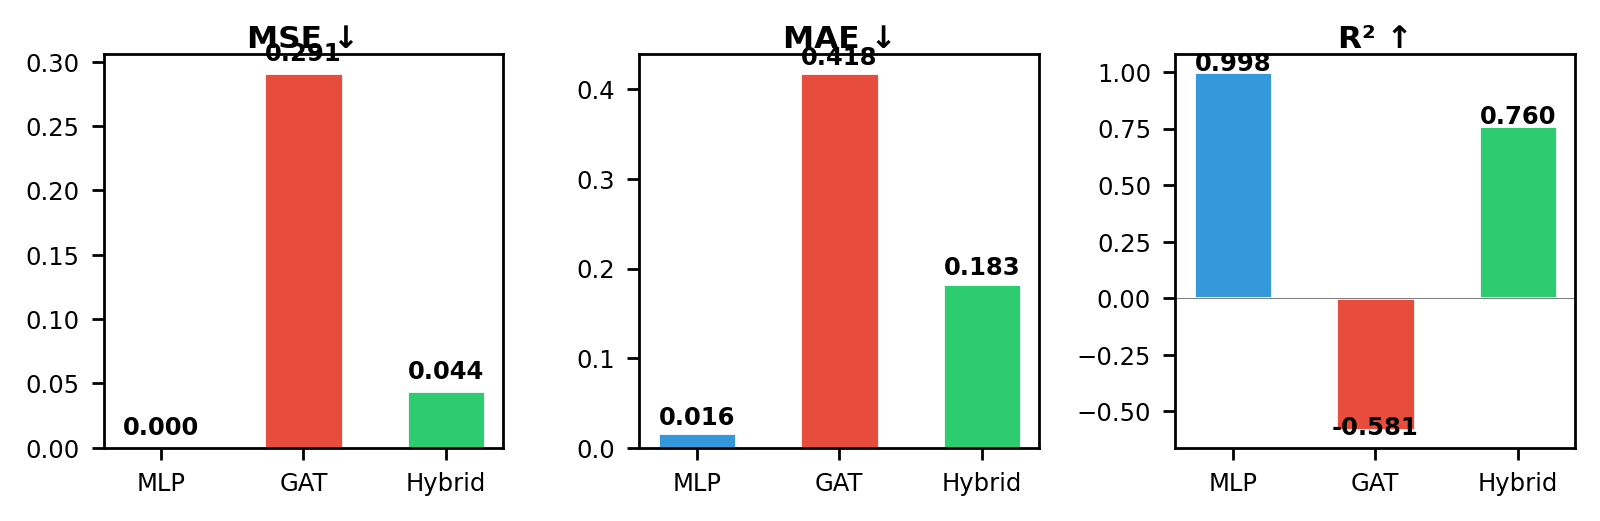
\includegraphics[width=\columnwidth]{results/figures/model_comparison.png}
\caption{Model performance comparison across three metrics.}
\label{fig:comparison}
\end{figure}

\begin{figure}[H]
\centering
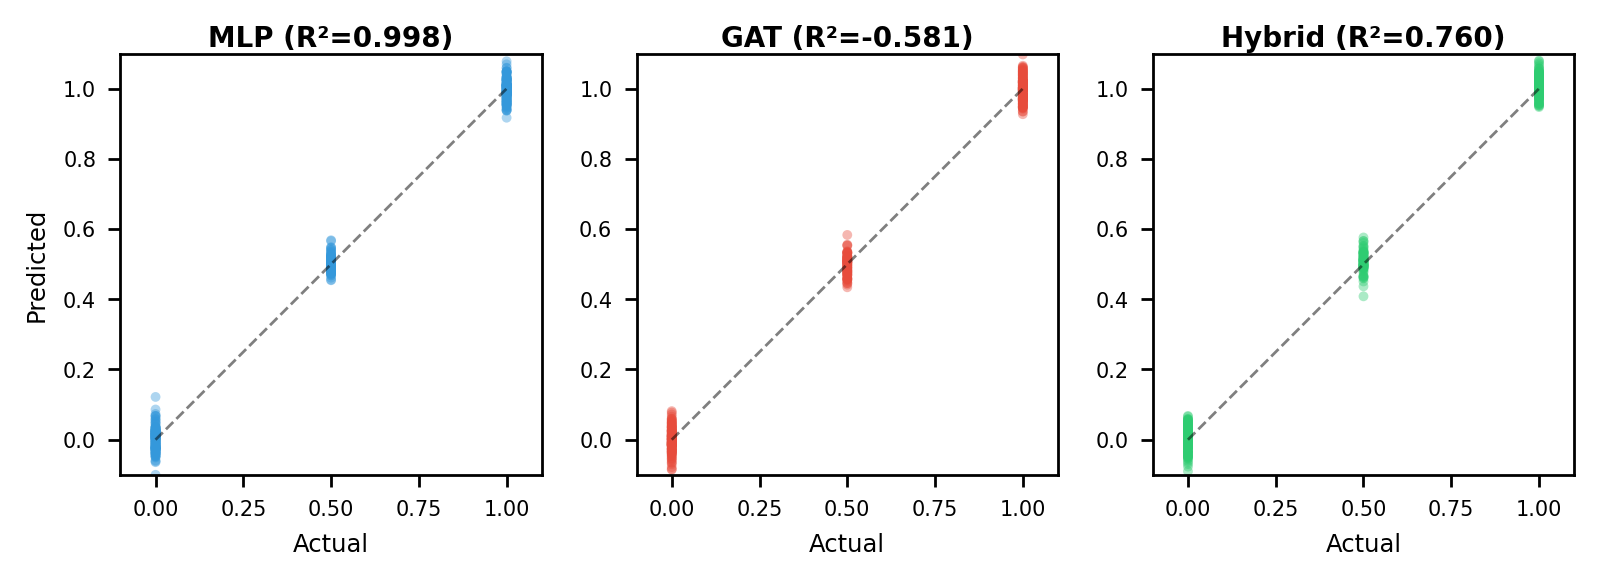
\includegraphics[width=\columnwidth]{results/figures/prediction_scatter.png}
\caption{Predicted vs.\ actual interpretability scores for each model on the test set.}
\label{fig:scatter}
\end{figure}

\subsection{Analysis}

The dominance of the Structural MLP yields an important insight: at moderate dataset scales ($\sim$375 graphs), \textit{domain-informed feature engineering substantially outperforms end-to-end learned representations}. Our 34 metrics---designed with knowledge of what makes circuits interpretable (tree-likeness, modularity, flow patterns)---encode precisely the right inductive biases. The GNN, lacking these priors, cannot discover equivalent representations from limited data. The Hybrid's improvement over the pure GNN ($R^2$: $-0.581 \to 0.760$) confirms that structural features provide critical signal the GNN leverages but cannot independently learn. At larger scales (thousands of real graphs), the GNN may close the gap, but at current scales, engineered features remain essential.

% ══════════════════════════════════════════════════════════
\section{Discussion}
% ══════════════════════════════════════════════════════════

\subsection{Key Findings}

This project demonstrates that structural properties of attribution graphs are highly predictive of interpretability quality. Tree-likeness, cycle density, modularity, and spectral gap form a core diagnostic suite that reliably distinguishes interpretable circuits from superposed ones. These metrics require only graph structure (not model internals), making them practical as automated diagnostics.

\subsection{Implications}

Our results suggest a practical workflow: after generating an attribution graph, compute structural metrics to quickly assess whether it will yield a clean circuit. Graphs with low tree-likeness, high cycle density, or low modularity indicate superposition and warrant caution. This pre-screening could save significant human analysis time on large-scale interpretability projects.

\subsection{Limitations}

Several limitations apply. (1) Synthetic labels are defined by construction, not expert judgment---real interpretability assessment is more nuanced. (2) Consumer hardware (M3 MacBook Pro) limited real graphs to $\sim$30; GPU clusters would enable larger-scale validation. (3) We analyzed a single model (Gemma-2-2B); results may differ for other architectures.

\subsection{Future Work}

Directions include: scaling to thousands of real graphs via GPU clusters; tracking interpretability changes during training (dynamics analysis); node-level superposition detection; and cross-model validation on Gemma-7B and Llama-70B to test scale invariance of structural signatures.

\subsection{Conclusion}

We present a novel application of data mining and graph neural networks to detecting superposition in attribution graphs. Our 34 structural metrics, combined with a hybrid GNN architecture, provide an automated, scalable approach to assessing interpretability quality, bridging graph mining research and mechanistic interpretability.

\subsection{Course Reflections}

This course gave me a strong appreciation for how broadly data mining techniques apply beyond traditional tabular datasets. The progression from foundational methods like KNN and decision trees through clustering and PCA to graph mining and neural networks felt very well structured---each topic built naturally on the last. The graph mining lectures were especially relevant to this project, as they gave me the vocabulary and tools to think about attribution graphs as objects worth mining in their own right. I also found the image and language mining modules eye-opening for understanding how the same core principles (feature extraction, similarity, dimensionality reduction) transfer across very different data modalities. Working on this project was the highlight of the course for me; applying what we learned in class to a real open problem in AI safety made the material feel immediately useful rather than purely academic. Overall, this was one of the most practically valuable courses I have taken.

% ══════════════════════════════════════════════════════════
\bibliographystyle{plainnat}
\begin{thebibliography}{10}

\bibitem{elhage2022superposition}
N.~Elhage et~al.
\newblock Toy models of superposition.
\newblock \textit{Anthropic Research}, 2022.

\bibitem{templeton2024scaling}
A.~Templeton et~al.
\newblock Scaling monosemanticity: Extracting interpretable features from {Claude} 3 {Sonnet}.
\newblock \textit{Anthropic Research}, 2024.

\bibitem{conerly2024circuit}
T.~Conerly et~al.
\newblock Update on circuit tracing: Improved attribution methods.
\newblock \textit{Anthropic Research}, 2024.

\bibitem{olah2020zoom}
C.~Olah et~al.
\newblock Zoom in: An introduction to circuits.
\newblock \textit{Distill}, 2020.

\bibitem{velickovic2018gat}
P.~Veli{\v{c}}kovi{\'c} et~al.
\newblock Graph attention networks.
\newblock In \textit{ICLR}, 2018.

\bibitem{kipf2017gcn}
T.~N. Kipf and M.~Welling.
\newblock Semi-supervised classification with graph convolutional networks.
\newblock In \textit{ICLR}, 2017.

\bibitem{blondel2008louvain}
V.~D. Blondel et~al.
\newblock Fast unfolding of communities in large networks.
\newblock \textit{J.\ Stat.\ Mech.}, 2008.

\bibitem{newman2006modularity}
M.~E.~J. Newman.
\newblock Modularity and community structure in networks.
\newblock \textit{PNAS}, 103(23):8577--8582, 2006.

\bibitem{fortunato2010community}
S.~Fortunato.
\newblock Community detection in graphs.
\newblock \textit{Physics Reports}, 486(3):75--174, 2010.

\bibitem{milo2002motifs}
R.~Milo et~al.
\newblock Network motifs: Simple building blocks of complex networks.
\newblock \textit{Science}, 298(5594):824--827, 2002.

\end{thebibliography}

\end{document}
